\documentclass[11pt, A4paper, english]{article}
\usepackage[utf8]{inputenc}
\usepackage[T1]{fontenc}
\usepackage{babel}
\usepackage{amsmath}
\usepackage{amsfonts}
\usepackage{amsthm}
\usepackage[colorlinks]{hyperref}
\usepackage{listings}
\usepackage[pdftex]{color}
\usepackage{hyperref}
\usepackage{graphicx}
\usepackage{cite}
\usepackage{float}
\usepackage{multicol}
\usepackage{subcaption}
\usepackage[margin=2cm]{geometry}

\definecolor{dkgreen}{rgb}{0,0.6,0}
\definecolor{gray}{rgb}{0.5,0.5,0.5}
\definecolor{daynineyellow}{rgb}{1.0,0.655,0.102}
\definecolor{url}{rgb}{0.1,0.1,0.4}

\lstset{
frame=tb,
language=Python,
aboveskip=3mm,
belowskip=3mm,
showstringspaces=false,
columns=flexible,
basicstyle={\small\ttfamily},
numbers=none,
numberstyle=\tiny\color{gray},
keywordstyle=\color{blue},
commentstyle=\color{daynineyellow},
stringstyle=\color{dkgreen},
breaklines=true,
breakatwhitespace=true,
tabsize=3
}

%The exemples under is for paths in windows and the second is in linux
\lstset{inputpath = /home/torstein/Dokumenter/UiO/Fys-Stk4155/"Python programmer"}

\graphicspath{{/home/torstein/Dokumenter/UiO/Fys-Stk4155/"Python programmer"/Results/}}
\hypersetup{colorlinks, urlcolor=url}

%This is how to put in codefiles
%\lstinputlisting{<Filnavn type kodefil>}
%To crope lines shown insert
%firstline = <linenumber>, lastline = <linenumber>
%as kwarg

%This is how to put in pictures
%\includegraphics[width=12.6cm,height=8cm]{<Filnavn type png>}
%To crop a picture insert 
%trim={<left> <lower> <right> <upper>}, clip
%as kwargs

\author{
Torstein Solheim Ølberg \\
Institute for Theoretical Astrophysics, University of Oslo \\
P.O. Box 1029 Blindern 0315 Oslo, Norway
%F.eks:
%Institute for Theoretical Astrophysics, University of Oslo \\
%P.O. Box 1029 Blindern 0315 Oslo, Norway
}
\title{Regression method on Star Formation of Galaxies Through Time}

\begin{document}
	
\maketitle
\tableofcontents
\clearpage
	
	\section{Abstract}
%Here the article is briefly summarized, mentioning some background, the methods and data used as well as notable results - keep it short and to the point.
The period of reionization is an important time stamp and period for the universe, where a large portion of matter changed from the neutral state present in the dark ages of the universe and to the ionized state we see a lot of today. Star formation has been speculated on being one of the mayor causes of this reionization, and in this article we will try to study if there are relations between the star formation rate and the time of the universe. We use data from the SDSS data release 7 and perform a Ordinary Least Squares, Ridge and Neural Network regression of about one hundredth of the amount of points in the data release. We find that there are some problems with the neural network setup, where it predicts the opposite of what we would expect, but end up with all three methods showing a relation between the redshift and Star formation rate. However without any error margins we can not conclude on anything, only further the interest in analysis for a larger timespan and a later data release like the SDSS dr16.
	
	
	\begin{multicols}{2}
		\section{Introduction}
%Why are we doing this exercise, what are our assumptions, what do we want to accomplish?
The topic of star formation rates for different galaxies is an interesting one, since star formation could be a factor in leading to the reionization of the universe some time at the end of the dark ages. Reionization is the time when the universe started to move from a mostly neutral state, where few particles interacted with each other to a universe full of the ionized matter we know today. It is important to understand this time of the universe, both because it is an important timestamp in cosmological models and to understand the objects we see today. \\
Most galaxies form stars in them, though some more than others. So called starburst galaxies can have many times higher rate of formation than what we are used to from our own Milky Way. If star formation is indeed a factor leading to reionization, then these galaxies would contribute much more to the reionization than other galaxies. \\
In this rapport we want to study the star formation rate of different galaxies through different regression methods and see if there is a relation between the starburst galaxies and the redshift, or time, of the universe. We will use two linear regression method, Ordinary Least Squares and Ridge, from \cite{Project 1} and a Neural Network we will try to build myself to look for relations between star formation rate and redshift. \\
First we will describe the dataset, then we will introduce the Neural network set up and the determination method for the best fit methods, then we will state the results, discuss them and try to conclude.
		
		\section{Data Description}
The data we will use is from the Sloan Digital Sky Survey (SDSS) \cite{SDSS} and their data release number 7. SDSS is a project with the goal of mapping most of the sky, measuring the intensity and redshift of most celestial objects. The data release 7 (dr7) contains over seven hundred thousand galaxy objects with their redshift, or timestamp, and the derived parameter SFR which is the amount of solar masses formed per year. We will use about every hundred galaxy, giving us about seven thousand data points, ranging from redshift around zeros, which is today, to redshift of about 0.7. For the neural network regression we will split the galaxies into two different categories, either with $SFR = 100$ or $SFR = 1$. We will do this by taking the integer division of the SFR with 50.

		\section{Methods}
%How did you obtain the data, what methods did you use? Describe your work process. If you performed an experiment using specific equipment, describe your setup.
The model used for the regression is the same as the one from \cite{Project 1} except we only have a one dimensional data set, which gives us the more simple model
			\begin{equation}
z = \sum_{i = 0}^{p} \beta_{i} x^{i}
			\end{equation}
where we choose the complexity degree p of the model.

			\subsection{Classification Neural Network}
A neural network is a program which simulates small components working together to perform a task. In our case this is to find a good fit for a dataset. This neural network is build up of different layers with a number of neurons. There are four different steps in this process, setting the activation function $f(x)$, calculating the initial bias and weights and then training the model through the feed forward and backward propagation methods. The activation function is a function used by each of the neurons to find the probability in the feed forward method. a normal function to use is the sigmoid function
				\begin{equation}
f(x) = \frac{1}{1 + e^{-x}}
				\end{equation}
which is practical to introduce non linearity into the program which would be lost if very simple methods are used. \\
Then the program can set up bias and weights where the weights are chosen randomly from a normal distribution and biases are set to a single value. Then the model is trained many times by drawing a random number of points from the dataset with replacement and the feed forward and backward propagation methods are called. \\
Feed forward method calculate
				\begin{equation}
g = w_l \circ X + b_l
				\end{equation}
where $w_l$ is the weights of the layer, $X$ is the data matrix and $b_l$ are the bias of the layer. Then it applies the activation function on $g$ and the result is multiplied by the last layer's weights and biases
				\begin{equation}
g_o = w_L \circ X + b_L
				\end{equation}
Then we can calculate the probability estimate of the categories we want the model to look for with
				\begin{equation}
P = \frac{e^{g_o}}{\sum_{i = 0}^{n} e^{g_o}}
				\end{equation}
With the backwards propagation method, we calculate the error if the probability was the true values, by withdrawing the training data points from the probabilities and then then using the result $h$ in the formula
				\begin{equation}
e = w_L^T \circ h \cdot f(g) (1 - f(g))
				\end{equation}
We calculate the gradient for the weights and the bias
				\begin{gather}
\nabla w_l = X^T \circ e \\
\nabla b_l = \sum e \\
\nabla w_L = h^T \circ f(g) \\
\nabla b_L = \sum h
				\end{gather}
These gradients are multiplied by a learning factor $\eta$ and then added to the former weights and biases. \\
When the model is trained, we can predict a function value $y$ by giving the feed forward a specific data matrix and we get the resulting probability distribution for the categories. We will use two categories, $SFR = 1$ or $SFR = 100$, and pick the numbers for our estimate randomly using this probability distribution. \\
We train the model $500$ times, with a learning factor of $\eta = 0.01$. We split our data into $80 \%$ training and $20 \%$ testing and find the complexity giving the best fit first. Then we use this to get a prediction using the whole $7000$ point dataset

				\subsection{Other regression methods methods}
We will follow the same method for Ridge and Ordinary Least Squares regression as in \cite{Project 1}. This is the standard OLS and Ridge regression methods and we choose a $\lambda = 1e-5$ for Ridge.

			\subsection{Analysis methods}
We need to find a way to measure which method is the best at approximating our dataset, and to do this a simple measure might be to look at the Mean Square Error and use this as our prediction error. \\
The MSE is simply the mean value of the square of the errors between the approximations and the measured values.
				\begin{equation}
MSE = \frac{1}{n} \sum_{i} \left( z_i - \hat{z}_i \right)^2
				\end{equation}
where $z$ are the measured values and $\hat{z}$ are the true values. \\

		\section{Results}
%What were your clear-cut results? - Present them in a clear and concise manner, waiting with the discussion of them for later. Here you present calculations, figures and tables of data, output of code, etc.
First we found the mean square estimate of the three regression methods. This gives us a plot of the MSE against the polynomial degree of the model.
			\begin{figure}[H]
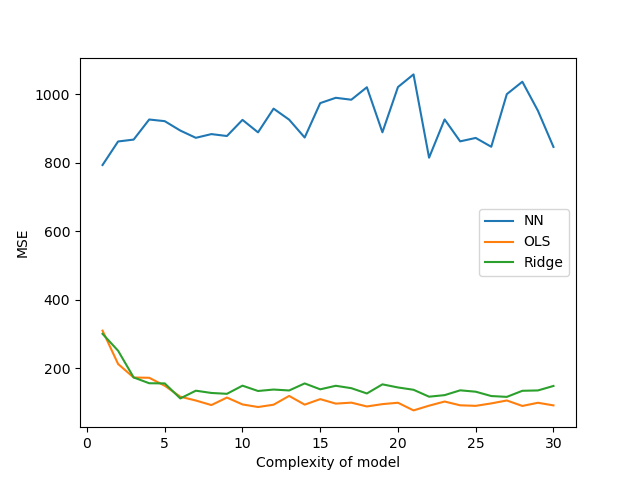
\includegraphics[width = 9.5cm, height = 8cm]{Figure1.png}
\caption{The Mean square estimate versus complexity for the Neural network classification, Ridge regression method and OLS method. We see that there is a large gap between the value for the neural network and the two other. The neural network method seem to stay quite constant for complexity but the OLS and Ridge are reduced until around complexity degree 10 and then seem to stabilise after this.}
\label{MSE}
			\end{figure}
The MSE plot in figure \ref{MSE} shows a large difference between the neural network and the other two methods with the neural network hovering a MSE between 800 and 1000 and the other two range from about 300 to around 100 or 150. We can also see that the MSE for the neural network varies a bit, but is approximately constant for all complexity degrees. However the other regression methods have a lower MSE for larger complexity until about a polynomial degree of 10, where it stabilises. \\
With the chosen polynomial degree taken from the MSE plot we find a model for all data points for all three regression method and plot the result in together with the measured data.
			\begin{figure}[H]
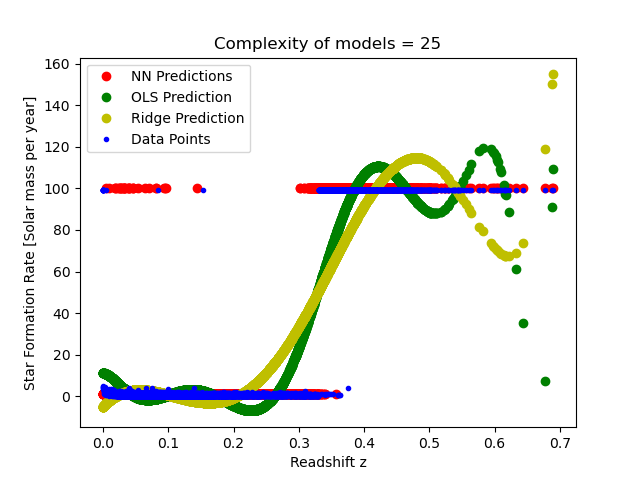
\includegraphics[width = 9.5cm, height = 8cm]{Figure2.png}
\caption{Here we see the three models and the data points we use. All three methods seem to change from a lower part for lower values of redshift, while for higher values the models seem to favour higher values of SFR. There also seem to be a change for even higher values of SFR at the end of the Ridge method and lower levels again for OLS just at the end.}
\label{Models}
The data models in figure \ref{Models} show a clear difference for low and high values of redshift for all three models. For low redshift the star formation rate is low and around redshift $0.3$ to $0.4$ the level changes to much higher and fluctuate around star formation rate of 100. In the end we see an indication of a change again in the two curve regression methods where Ridge regression seem to rise for even higher values and OLS seem to change back down to where is was before.
			\end{figure}

		\section{Discussion}
%Were the results what you expected? Are the results significant? - meaning; are the results clear, or are they open to interpretation? How certain can you be of them? What do these results mean in a wider context?
Along the way we encountered a problem with the neural network, where it seem to give a very high MSE of about $8000$. When we plotted it there seem to be a complete reversal of where it placed the predicted points as supposed to where the data points where located. However if we reversed the probability calculation done in the final feed forward method when predicting the data, this problem was solved. However, why this would be the case in the first place we do not know since this is simply the derivative of the activation function and taking the reversal is just subtracting it from one. However this might indicate there is something wrong with the mathematical construction of my neural network however the program predicts very nicely the points it is supposed to. \\
The mean square estimate for the model of the neural network is as mentioned much larger than for the other regression methods. This is probably a result of this method being a classification method using only two categories instead of a curve regression method like the two others where the method can give many different values instead of just two. The fact that it doesn't seem to be dependant on complexity degree in any obvious way could be an indication of the dataset only needing a very simple model to be predicted accurately, but overfitting doesn't seem to be a very large problem either. \\
From the MSE analysis we see that the complexity degree of 25 seem to give a fine value in all three methods and we choose this value. However, any value after the 10th could also be good however 25 is in one of the seemingly random valleys of the neural network curve. \\
We have not included any error estimates in the methods which we could take from the dataset or any estimate errors for the regression models which would give us error bars for each model. This would not have been an easy thing to do for the neural network, but would have been possible for the regression methods to do. However, the goal of our analysis was simply to get a feel of if there where any relation between the time and the amount of star burst galaxies, and we thought it sufficient to only see if the methods favoured any values at different times. There could always be that the error estimates are to large for us to properly conclude on anything definitely, but this is also not our mission. \\
In the end there seem to be some relation between the redshift and the star burst galaxies for all the methods, with more star burst galaxies later in time than earlier. Only the neural network predicts a portion of star burst galaxies at low redshift, but this amount is only in the beginning and then disappear after redshift of about $0.1$. Even thought this is the results we had hoped for, there are other explanations and problems. First of all there might be that star burst galaxies are much easier to observe for higher redshift, and that they thus show up more, the complete lack of normal galaxies in the dataset for the higher values of redshift is very suspicious in this way. There is also the problem that reionization takes place at even higher redshift that this, or longer back in time, but since the goal of this paper was just to find an indication of relation between star burst galaxies and time, this is not direct problem. However, it means that there are more to be done before we can conclude on any relation between the star formation and reionization.

		\section{Conclusion}
As we have seen there where some odd consequence of the construction of the neural network, but the method shows the same as the other regression methods which is that there are some relation between star formation rate and redshift. Though there are no error estimates in our analysis and the results can be explained by some other factors there is reason to believe further investigation of star burst galaxies, particularly for higher redshift and also with error estimates would be interesting. There are also newer data releases which are harder to access from the SDSS, with the latest being the dr16 with more than 5 times as many objects as we had access to and ranging all the way back to redshift $z = 7$.

		
\addcontentsline{toc}{section}{Bibliography}
		\begin{thebibliography}{9}
			\bibitem{Project 1}
On Linear Regression Methods for a Terrain Dataset; \\
Torstein Solheim Ølberg \\
\url{https://github.com/MrTorstein/Fys-Stk4155}
Published 10/10-2020 \\
Downloaded 10/10-2020
			\bibitem{SDSS}
Sloan Digital Sky Survey; \\
Sloan Digital Sky Survey/SkyServer \\
\url{http://cas.sdss.org/dr7/en/} \\
Published: 1/08-2013 \\
Downloaded: 1/12-2020
		\end{thebibliography}
	\end{multicols}
\end{document}